\documentclass[aps,prx,reprint,notitlepage,nofootinbib]{revtex4-2}
\usepackage[T1]{fontenc}
\usepackage{lmodern}
\usepackage{amsmath,amssymb,amsthm,bm,mathtools,mathrsfs}
\usepackage{graphicx,xcolor,booktabs,tabularx,array,multirow}
\usepackage{tikz,pgfplots}
\usepackage{microtype}
\usepackage{hyperref}
\usetikzlibrary{arrows.meta,positioning,calc,fit,decorations.pathreplacing}
\pgfplotsset{compat=1.18}
\begin{document}
\title{Portable scientific typesetting smoke test}
\date{}
\begin{abstract}Public dependency and font test.\end{abstract}
\maketitle
\section{Mathematics}\label{sec:math}
\begin{align}
\mathcal N_\gamma&=(1-\gamma)\operatorname{id}+\gamma\mathcal R_{I/2},\label{eq:noise}\\
m_T&\ge a\left[D\kappa-\ln(2n/a)\right]_+ .
\end{align}
\textbf{Bold}, \textit{italic}, \texttt{monospace},
$\mathbf{x}$, $\bm\sigma$, $\mathbb C$, $\mathfrak A$, $\mathscr A$,
$\sum_{j=0}^{D}\prod_{i=1}^{n}q_i$,
$\frac12\lVert\Lambda-\mathrm{id}\rVert_\diamond$.
\begin{figure}[ht]
\centering
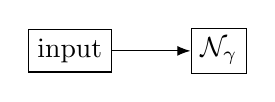
\begin{tikzpicture}[node distance=1cm]
\node[draw] (a) {input};\node[draw,right=of a] (b) {$\mathcal N_\gamma$};
\draw[-{Latex}] (a)--(b);
\end{tikzpicture}
\caption{Public schematic smoke test.}\label{fig:smoke}
\end{figure}
\begin{table}[ht]\caption{Font test.}\label{tab:smoke}\begin{ruledtabular}
\begin{tabular}{cc}Resource&Count\\\hline Width&$n$\\Work&$m_T$\end{tabular}
\end{ruledtabular}\end{table}
\appendix\section{Auxiliary mathematics}
$\alpha=\log_2 5$, $\ell=1+\ln[k(\gamma D+1)/\epsilon]$.
Section~\ref{sec:math}, Eq.~\eqref{eq:noise}, Fig.~\ref{fig:smoke},
and Table~\ref{tab:smoke} exercise cross-reference destinations.
An ordinary citation~\cite{test} and \url{https://journals.aps.org/prxquantum/}
exercise bibliography and URL links.
\begin{thebibliography}{1}
\bibitem{test}A. Author, Public smoke test (2026).
\end{thebibliography}
\end{document}
